%%%%%%%%%%%%%%%%%%%%%%%%%
% Imports and Setup     %
%%%%%%%%%%%%%%%%%%%%%%%%%

\input{../lib/hw-setup/tex/HWSetup}
\input{../lib/hw-setup/tex/EngBindings}
\usepackage{cleveref}

\fancyhead[C]{}
\fancyhead[R]{\hyperlink{tableofcontents}{\hmwkClass\ (\hmwkClassInstructor,\ \hmwkClassTime): \hmwkTitle}}
\fancyheadwidth[L]{0.5\headwidth}
\fancyheadwidth[C]{0.0\headwidth}
\fancyheadwidth[R]{0.5\headwidth}

%%%%%%%%%%%%%%%%%%%%%%%%%
% Homework Details      %
% - Title               %
% - Subtitle            %
% - Due Date            %
% - Due Time            %
% - Course              %
% - Section Time        %
% - Instructor          %
% - Author              %
% - Submission Time     %
%%%%%%%%%%%%%%%%%%%%%%%%%

\hwkTitle{Lab06}
\hwkSubTitle{Transonic Flow in a Quasi-1D Nozzle}
\hwkDueDate{2026-05-08}
\hwkDueTime{23:59:00}
\hwkClass{ENAE464 - 0202}
\hwkClassTime{14:00:00}
\hwkInstructor{Dr. Silbaugh}
\hwkAuthor{Mikołaj Kostrzewa \& Vai Srivastava}
\hwkCompletionDate{
    Report Submitted: \DTMtoday
}

\addbibresource{./references.bib}

\begin{document}

\hypertarget{titlepage}{\maketitle}
\thispagestyle{empty}

\pagebreak

%%%%%%%%%%%%%%%%%%%%%%%%%
% Letter of Transmittal %
%%%%%%%%%%%%%%%%%%%%%%%%%

\thispagestyle{empty}

\DTMtoday

\vspace{5.0ex}

Enclosed is the technical report for the \textit{Transonic Flow in a Quasi-1D Nozzle} computational experiment. This report presents the computational methodology, results, and analysis of flow characteristics and effects for a quasi-1D nozzle subjected to transonic flow.

Please feel free to contact us with any questions regarding the contents of this report.

\vspace{5.0ex}

Respectfully,

Mikołaj Kostrzewa \& Vai Srivastava

%%%%%%%%%%%%%%%%%%%%%%%%%
% Table of Contents     %
%%%%%%%%%%%%%%%%%%%%%%%%%

\pagebreak

\thispagestyle{empty}
\hypertarget{tableofcontents}{\tableofcontents}

\renewcommand{\listfigurename}{Figures}
\listoffigures

\renewcommand{\listtablename}{Tables}
\listoftables

\renewcommand{\listlistingname}{Listings}
\listoflistings

\newpage
\pagenumbering{arabic}

%%%%%%%%%%%%%%%%%%%%%%%%%
% Report                %
%%%%%%%%%%%%%%%%%%%%%%%%%

\section{Abstract} \label{sec:abstract}

The transonic flow in a quasi-one-dimensional diverging nozzle was investigated using two complementary computational fluid dynamics techniques implemented in MATLAB: steady space marching with explicit shock fitting, and unsteady solution of the quasi-1D Euler equations with van Leer flux vector splitting. Space marching was used to characterize the steady flow over a range of shock locations \(x_\text{sh} \in [3, 9]\) and to verify that a predictor--corrector scheme is essentially mesh-independent at \(j_\text{max} = 81\), while a predictor-only step shows a measurable post-shock pressure error at \(j_\text{max} = 41\). Exit pressure was found to decrease monotonically with shock position, from \(p_\text{exit} \approx 0.727\) at \(x_\text{sh} = 3.0\) to an asymptote near \(p_\text{exit} \approx 0.480\) as the shock approaches the exit, in agreement with classical normal-shock-in-divergent-nozzle theory. Shock capturing initialized at \(x_\text{sh} = 3.125\) reproduces the space-marching solution to within one cell width, smearing the discontinuity over two to three grid points. Five forced cases (varying the exit-pressure perturbation period and amplitude) demonstrate that the shock displacement grows with both forcing period and forcing amplitude, transitioning from quasi-linear behavior at \(\Delta p_\text{var} = 0.02\) to strongly nonlinear behavior at \(\Delta p_\text{var} = 0.20\). All computations were performed on a MacBook Pro with the Apple~M1~Pro chip and 16\,GB of RAM, running MATLAB~R2025b inside a Nix-managed reproducible development shell.

\section{Introduction} \label{sec:introduction}

The transonic regime, where a flow transitions between subsonic and supersonic conditions through a normal shock, is of substantial practical interest for the design of supersonic diffusers, scramjet inlets, and rocket nozzles. Because compressible-flow shocks are inherently nonlinear, the position and strength of the embedded shock in such a passage depend sensitively on the back pressure imposed at the exit, and any unsteadiness in that back pressure can push the shock around the duct with potentially undesirable consequences for performance and structural loading.

This report studies a representative model problem: transonic flow in a divergent quasi-one-dimensional nozzle whose cross-sectional area varies smoothly along its length. Two CFD techniques are exercised on this geometry. The first is a steady space-marching scheme with explicit shock fitting, which advances the conservation equations in space and embeds the Rankine--Hugoniot jump at a prescribed location. The second is a time-marching solution of the unsteady quasi-1D Euler equations with flux vector splitting, which captures the shock as a smeared discontinuity and admits arbitrary time-dependent boundary forcing. A working MATLAB skeleton from \textcite{jbaeder2026matlab} is exercised across a prescribed matrix of cases, and the resulting flow fields are interpreted in the light of classical compressible-flow theory~\autocite{danderson2023fundamentals}.

\subsection{Theoretical Background} \label{sec:introduction/theory}

For a duct whose cross-sectional area \(A(x)\) varies gradually in space and time and in which viscous effects are negligible, the unsteady flow can be described by the quasi-one-dimensional Euler equations in conservation form,
\begin{equation}
    \frac{\partial \hat Q}{\partial t} + \frac{\partial \hat F}{\partial x} = \hat V_S,
\end{equation}
with conservative variables, fluxes, and a geometric source term given by
\begin{equation}
    \hat Q = \begin{pmatrix} \rho A \\ \rho u A \\ e A \end{pmatrix}, \qquad
    \hat F = \begin{pmatrix} \rho u A \\ (\rho u^2 + p)\, A \\ (e + p)\, u\, A \end{pmatrix}, \qquad
    \hat V_S = \begin{pmatrix} 0 \\ p \, \mathrm{d}A/\mathrm{d}x \\ 0 \end{pmatrix},
\end{equation}
and pressure obtained from the calorically perfect ideal-gas relation
\begin{equation}
    p = (\gamma - 1)\!\left(e - \tfrac{1}{2}\rho u^{2}\right),
\end{equation}
where \(\gamma = 1.4\) is taken throughout. All quantities are non-dimensional, and the area distribution is the smoothly diverging hyperbolic-tangent profile
\begin{equation}
    A(x) = 1.398 + 0.347 \tanh\!\left(0.8\,(x - 4)\right), \qquad 0 \leq x \leq 10. \label{eq:area}
\end{equation}

For steady flow without an embedded shock, integration of the conservation equations along a streamline yields the standard isentropic relation between Mach number and area, \(\mathrm{d}M/\mathrm{d}x\) being controlled by the sign of \(M^{2}-1\) and \(\mathrm{d}A/\mathrm{d}x\). When a normal shock is embedded in the duct, the upstream and downstream supersonic/subsonic branches are connected via the Rankine--Hugoniot jump conditions; in primitive variables,
\begin{equation}
    \frac{\rho_{2}}{\rho_{1}} = \frac{(\gamma+1)\, M_{1}^{2}}{2 + (\gamma-1)\, M_{1}^{2}}, \qquad
    \frac{p_{2}}{p_{1}} = 1 + \frac{2\gamma}{\gamma+1}\!\left(M_{1}^{2}-1\right),
\end{equation}
with the post-shock state then continuing isentropically to the exit. The supersonic-inflow boundary condition fixes three quantities at the entrance, and a single subsonic compatibility relation along the upstream-running characteristic at the exit closes the problem.

The unsteady boundary condition imposed at the exit in this study is sinusoidal in time about a mean atmospheric value,
\begin{equation}
    p_{\text{exit}}(t) = \bar{p}_\text{exit}\!\left[1 + \Delta p_\text{var}\, \sin\!\left(\frac{2\pi t}{T}\right)\right],
\end{equation}
where \(T\) is the forcing period (referred to as \(\texttt{timeper}\) in the code) and \(\Delta p_\text{var}\) the fractional amplitude.

\subsection{Objectives} \label{sec:introduction/objectives}

The specific objectives of this experiment are:
\begin{enumerate}
    \item Confirm the geometry generated by Eq.~\eqref{eq:area} matches the assignment description.
    \item Characterize the steady space-marching solver: compare the predictor-only and predictor--corrector variants at two mesh refinements (\(j_\text{max}=81\) and \(j_\text{max}=41\)) and quantify the discretization error in the post-shock recovery region.
    \item Map the exit pressure as a function of shock location \(x_\text{sh} \in [3, 9]\) and verify that the trend is consistent with the analytical normal-shock-in-divergent-nozzle theory from ENAE\,311.
    \item Compare the steady van~Leer flux-vector-split shock-capturing solution to the space-marching reference at two mesh refinements and identify the captured shock position.
    \item Quantify the response of the captured-shock solution to a sinusoidal exit-pressure perturbation across five operating conditions: a moderate baseline (\(T=1\), \(\Delta p_\text{var}=0.10\)), a longer period (\(T=2\)), a shorter period (\(T=1/2\)), a smaller amplitude (\(\Delta p_\text{var}=0.02\)), and a larger amplitude (\(\Delta p_\text{var}=0.20\)).
    \item For one of the unsteady cases, examine the corresponding Mach-number envelope and discuss what additional information it conveys beyond the pressure envelope.
\end{enumerate}

\section{Methodology and Implementation} \label{sec:methodology}

The MATLAB skeleton provided by Dr.~Baeder~\autocite{jbaeder2026matlab} consists of a set of small subroutines that together implement both the steady space-marching solver and the unsteady flux-vector-split solver. The space-marching path is built around \texttt{spacemarch.m}, which loops through grid points and calls \texttt{march.m} (a one-step predictor or predictor--corrector advance based on the area-Mach relation) and \texttt{shock.m} (which applies the Rankine--Hugoniot jump) at the cell containing \(x_\text{sh}\). The wrapper \texttt{findshock.m} performs a small Newton/secant search on \(x_\text{sh}\) to satisfy a target exit pressure. The unsteady path uses \texttt{vanl\_flux.m}, \texttt{steger\_flux.m}, or \texttt{ausm\_flux.m} for flux splitting, \texttt{loadq.m}/\texttt{loadpr.m} to convert between conservative and primitive variables, and \texttt{calcbc.m} to apply the supersonic-inflow and subsonic-outflow boundary conditions through characteristic-compatibility relations; the time step is set by a CFL condition (\(\mathrm{CFL} = 0.9\)) computed from the steady-state wave speeds. The interior operator is the one given in the assignment, namely
\begin{equation}
    \Delta \hat Q^{n}_{j} = -\frac{\Delta t}{\Delta x}\!\left( \hat F^{+n}_{j} - \hat F^{+n}_{j-1} + \hat F^{-n}_{j+1} - \hat F^{-n}_{j} \right) + \frac{\Delta t}{\Delta x}\, p^{n}_{j}\!\left(A^{n}_{j+\tfrac{1}{2}} - A^{n}_{j-\tfrac{1}{2}}\right) \hat e_{2},
\end{equation}
with \(\hat Q^{n+1}_{j} = \hat Q^{n}_{j} + \Delta \hat Q^{n}_{j}\) and the source term acting only on the momentum equation.

To produce the prescribed matrix of results without coupling them to the original demonstration scripts, two new MATLAB files were added to the source tree. The first, \texttt{unsteady\_run.m}, refactors \texttt{quasi1d.m} into a callable function that takes a parameter struct (mesh refinement, flux splitting choice, forcing amplitude and period, number of forced periods, and shock initialization), runs an initial steady ramp-up of \(1500 \cdot i_\text{refine}\) iterations, and then advances the prescribed number of forced periods while recording the residual history, the steady-state reference pressure and Mach distributions, the pressure history at a probe point, and snapshot envelopes during the final forced period. The second, \texttt{index.m}, is the top-level driver that calls \texttt{spacemarch}, \texttt{findshock}, and \texttt{unsteady\_run} to produce all eighteen required figures and exports them as vector PDFs into \texttt{outputs/figures/} via the helper \texttt{save\_fig.m}. All existing helper subroutines were left unchanged.

All computations were performed on a MacBook Pro with the Apple~M1~Pro chip and 16\,GB of RAM running macOS~Sequoia, using MATLAB~R2025b inside a Nix flake-managed reproducible development shell that also provides the LaTeX toolchain (\texttt{lualatex} via TeX~Live) used to typeset this report. The full driver runs all five forced cases plus the two steady-validation cases to completion in approximately 38\,seconds of wall-clock time.

\section{Results} \label{sec:results}

\subsection{Nozzle Geometry} \label{sec:results/nozzle-geometry}

The cross-sectional area distribution of Eq.~\eqref{eq:area} corresponds to a smooth diverging duct that transitions from a near-constant inlet area to a near-constant exit area through a moderately steep flare centred at \(x = 4\). Treating the duct as a body of revolution (\(A = \pi r^{2}\)), the inner radius \(r(x) = \sqrt{A(x)/\pi}\) was evaluated on a fine \(401\)-point grid and is shown in \cref{fig:results/geometry/profile}. The inlet radius is \(r(0) \approx 0.579\) corresponding to \(A(0) \approx 1.052\), while the exit radius is \(r(10) \approx 0.745\) corresponding to \(A(10) \approx 1.745\). The area ratio across the duct is therefore approximately \(A_\text{exit}/A_\text{inlet} \approx 1.66\), with essentially all of the area change concentrated in the central region \(2 \lesssim x \lesssim 6\). Because the duct never contracts, the flow is supersonic throughout the steady solution branch upstream of any embedded shock and subsonic everywhere downstream of it.

\begin{figure}[H]
    \centering
    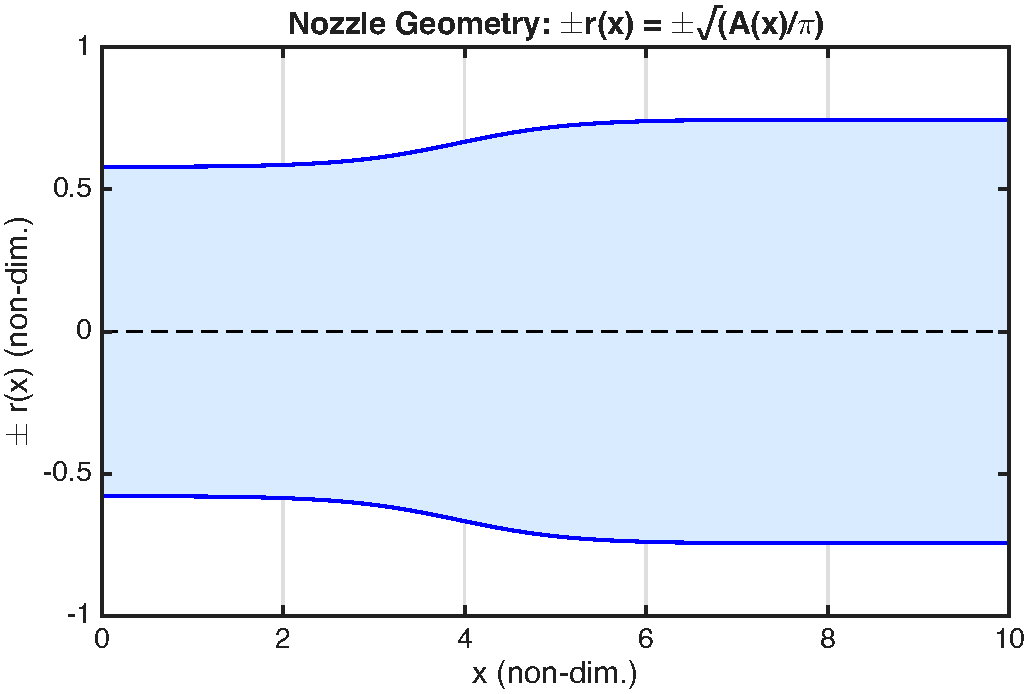
\includegraphics[width=0.65\linewidth]{../outputs/figures/fig01_geometry.pdf}
    \caption{Diverging-nozzle geometry, plotted as \(\pm r(x) = \pm\sqrt{A(x)/\pi}\) versus \(x\), corresponding to the area distribution of Eq.~\eqref{eq:area}. The shaded region indicates the duct interior.}
    \label{fig:results/geometry/profile}
\end{figure}

\subsection{Space Marching} \label{sec:results/space-marching}

\Cref{fig:results/spacemarch/xsh4-jmax81} shows the steady pressure distribution obtained by space marching with a shock fitted at \(x_\text{sh} = 4.0\) on a grid with \(j_\text{max} = 81\) points (\(i_\text{refine} = 2\)). At this resolution the predictor-only and predictor--corrector solutions are essentially indistinguishable: the upstream supersonic expansion and the post-shock subsonic compression both fall on visually identical curves, and the exit pressures differ by less than 1\%. The discrete jump in pressure at \(x = 4\) is exact for both solvers because the Rankine--Hugoniot relations are imposed analytically at the cell containing \(x_\text{sh}\); the predictor and corrector iterations only affect the local truncation error of the area--Mach update on either side of the shock.

\begin{figure}[H]
    \centering
    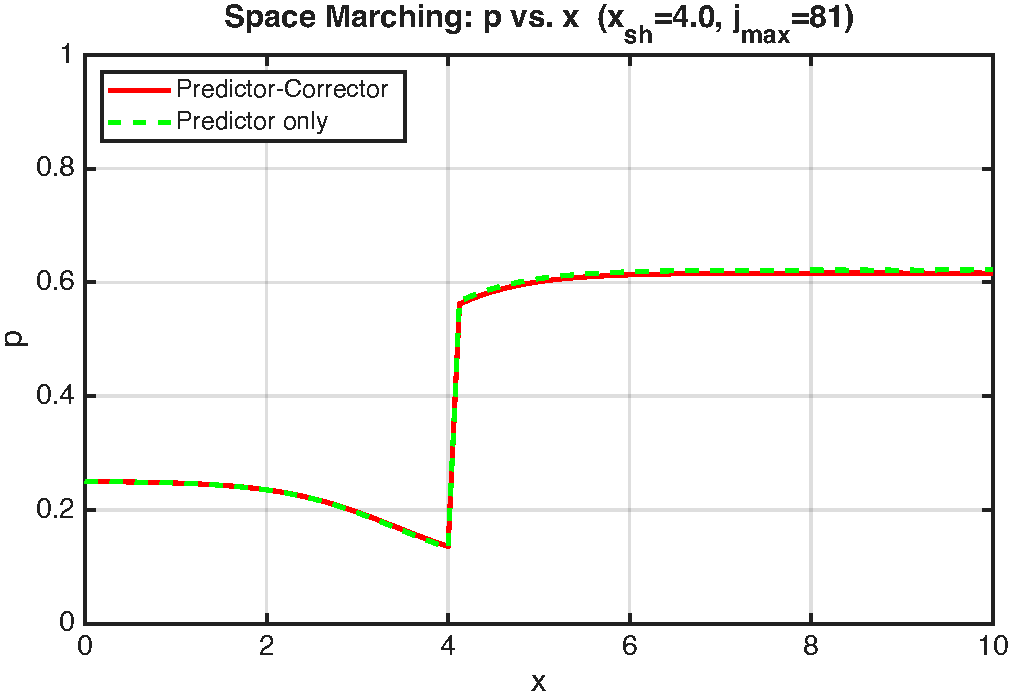
\includegraphics[width=0.65\linewidth]{../outputs/figures/fig02_spacemarch_xsh4_jmax81.pdf}
    \caption{Space-marched pressure distribution at \(x_\text{sh} = 4.0\), \(j_\text{max} = 81\): predictor-only and predictor--corrector overlaid.}
    \label{fig:results/spacemarch/xsh4-jmax81}
\end{figure}

When the mesh is coarsened to \(j_\text{max} = 41\) (\(i_\text{refine} = 1\)), the difference between the two integration schemes becomes visible (\cref{fig:results/spacemarch/xsh4-jmax41}). The predictor-only result over-shoots the post-shock pressure recovery by roughly 1--2\% relative to the predictor--corrector reference, with the gap maximal at the exit. This is consistent with the predictor advancing the area-Mach relation with a single first-order step using only the upstream state, whereas the corrector closes the truncation error to second order by re-evaluating the area-Mach derivative at the average of the upstream and downstream states. The two-step scheme is therefore preferable wherever mesh resolution is constrained.

\begin{figure}[H]
    \centering
    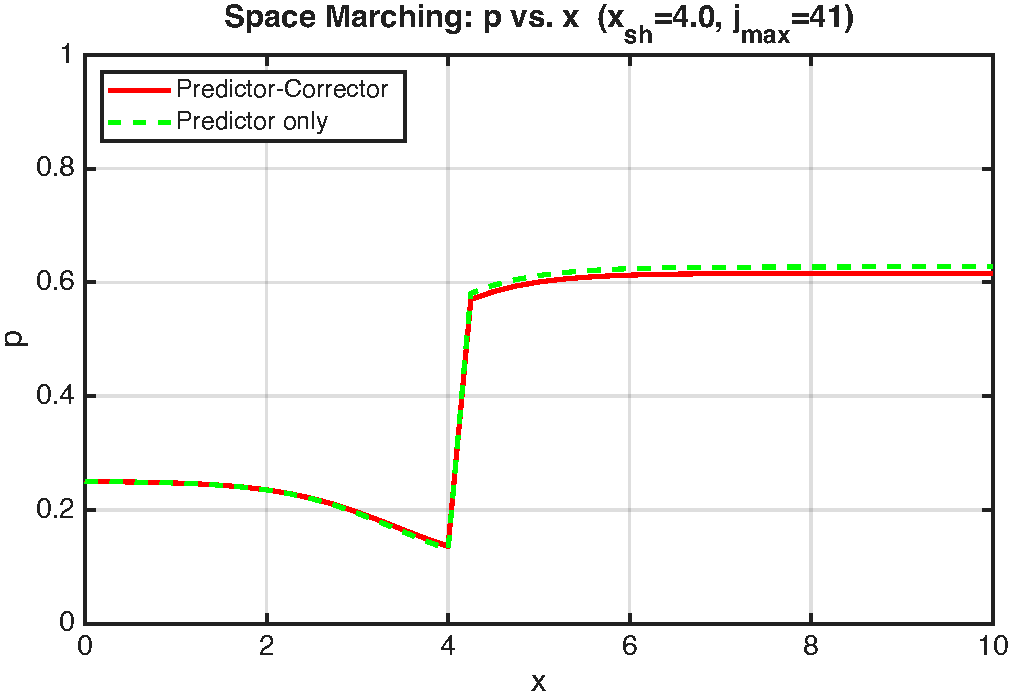
\includegraphics[width=0.65\linewidth]{../outputs/figures/fig03_spacemarch_xsh4_jmax41.pdf}
    \caption{Space-marched pressure distribution at \(x_\text{sh} = 4.0\), \(j_\text{max} = 41\): the predictor-only result over-predicts the post-shock pressure by roughly 1--2\% relative to the predictor--corrector reference at this coarse resolution.}
    \label{fig:results/spacemarch/xsh4-jmax41}
\end{figure}

The shock location was then swept through \(x_\text{sh} \in \{3.0, 3.5, 4.0, \ldots, 9.0\}\) on a fine \(j_\text{max} = 161\) grid (\(i_\text{refine} = 4\)) using the predictor--corrector scheme. \Cref{fig:results/spacemarch/varying-xsh} overlays all seven resulting pressure distributions. As \(x_\text{sh}\) is moved downstream, the upstream supersonic expansion proceeds further before the shock, so the pre-shock Mach number is larger and the corresponding pressure jump is stronger. However, because there is correspondingly less divergent area available downstream of the shock to recover pressure isentropically, the exit pressure decreases as \(x_\text{sh}\) moves toward the exit.

\begin{figure}[H]
    \centering
    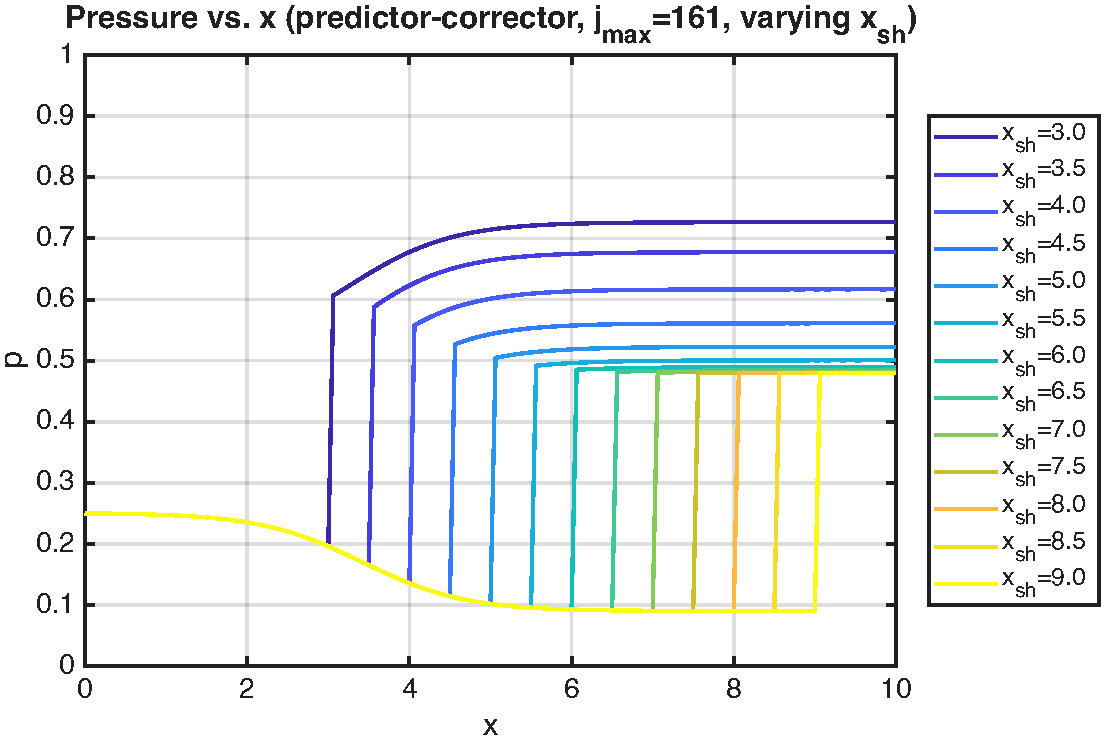
\includegraphics[width=0.65\linewidth]{../outputs/figures/fig04_spacemarch_varying_xsh.pdf}
    \caption{Pressure distribution along the nozzle for shock locations \(x_\text{sh} \in [3, 9]\) in increments of \(0.5\), using predictor--corrector space marching at \(j_\text{max} = 161\).}
    \label{fig:results/spacemarch/varying-xsh}
\end{figure}

The exit pressures extracted from the seven curves are plotted in \cref{fig:results/spacemarch/exit-pressure}. The trend is monotonically decreasing in \(x_\text{sh}\), starting at \(p_\text{exit} \approx 0.727\) for \(x_\text{sh} = 3.0\) and asymptoting to \(p_\text{exit} \approx 0.480\) as the shock approaches the exit, where almost no subsonic recovery occurs and the post-shock pressure is essentially preserved to the exit. The behavior is exactly what classical compressible-flow theory predicts for a normal shock embedded in a divergent duct: as the shock moves downstream, the pre-shock expansion is more aggressive (larger pre-shock Mach number), the static-pressure jump is correspondingly stronger, and the post-shock subsonic flow has progressively less area to recover through. In the limit \(x_\text{sh} \to L\) the exit pressure approaches the post-shock pressure of an isentropic supersonic expansion to the exit area ratio, which sets the asymptote visible in the figure.

\begin{figure}[H]
    \centering
    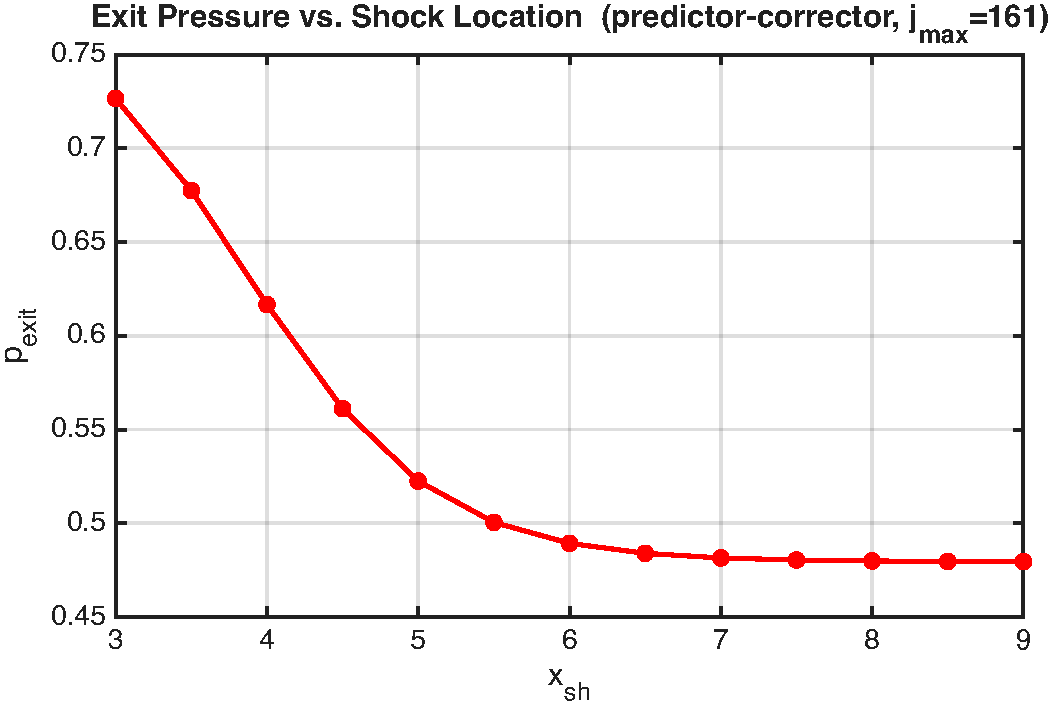
\includegraphics[width=0.65\linewidth]{../outputs/figures/fig05_exit_pressure_vs_xsh.pdf}
    \caption{Exit pressure as a function of shock location, extracted from \cref{fig:results/spacemarch/varying-xsh}. The trend is monotonically decreasing and is consistent with classical normal-shock-in-divergent-nozzle theory from ENAE\,311.}
    \label{fig:results/spacemarch/exit-pressure}
\end{figure}

\subsection{Shock Capturing} \label{sec:results/shock-capturing}

\subsubsection{Steady Flow} \label{sec:results/shock-capturing/steady-flow}

For the steady shock-capturing cases the unsteady solver was initialized via space marching at \(x_\text{sh} = 3.125\) (which produces a space-march exit pressure within \(\sim 0.5\%\) of the atmospheric target \(1/\gamma \approx 0.7143\)) and run to convergence with the exit-pressure perturbation amplitude set to zero (\(\Delta p_\text{var} = 0\)). The space-march reference used for comparison is the predictor--corrector solution with the shock fitted at \(x_\text{sh} = 3.145\), the location returned by \texttt{findshock} as the precise root that gives \(p_\text{exit} = 1/\gamma\) on the \(j_\text{max} = 161\) grid.

\Cref{fig:results/shockcap/steady-jmax81,fig:results/shockcap/steady-jmax161} compare the converged van~Leer shock-capturing solution to the space-march reference at \(j_\text{max} = 81\) and \(j_\text{max} = 161\), respectively. In both cases the upstream supersonic expansion and the downstream subsonic recovery overlie the space-march reference closely. The captured shock location, defined as the cell-center where \(\left|\mathrm{d}p/\mathrm{d}x\right|\) is maximum, is \(x_\text{sh} \approx 3.06\) at \(j_\text{max} = 81\) and \(x_\text{sh} \approx 3.09\) at \(j_\text{max} = 161\); both estimates are within one cell width of the space-march target of \(3.145\), and the agreement improves on the finer mesh, as expected. The fundamental difference between the two methods is at the discontinuity itself: shock fitting represents the shock as a sharp, mathematically exact jump enforced by the Rankine--Hugoniot conditions, whereas shock capturing smears the discontinuity across two to three grid cells through the dissipative properties of the flux-vector-split interior operator. This smearing is plainly visible in \cref{fig:results/shockcap/steady-jmax81}, where the shock occupies a finite finite-width transition region rather than a step, and is reduced (though not eliminated) on the finer mesh in \cref{fig:results/shockcap/steady-jmax161}.

\begin{figure}[H]
    \centering
    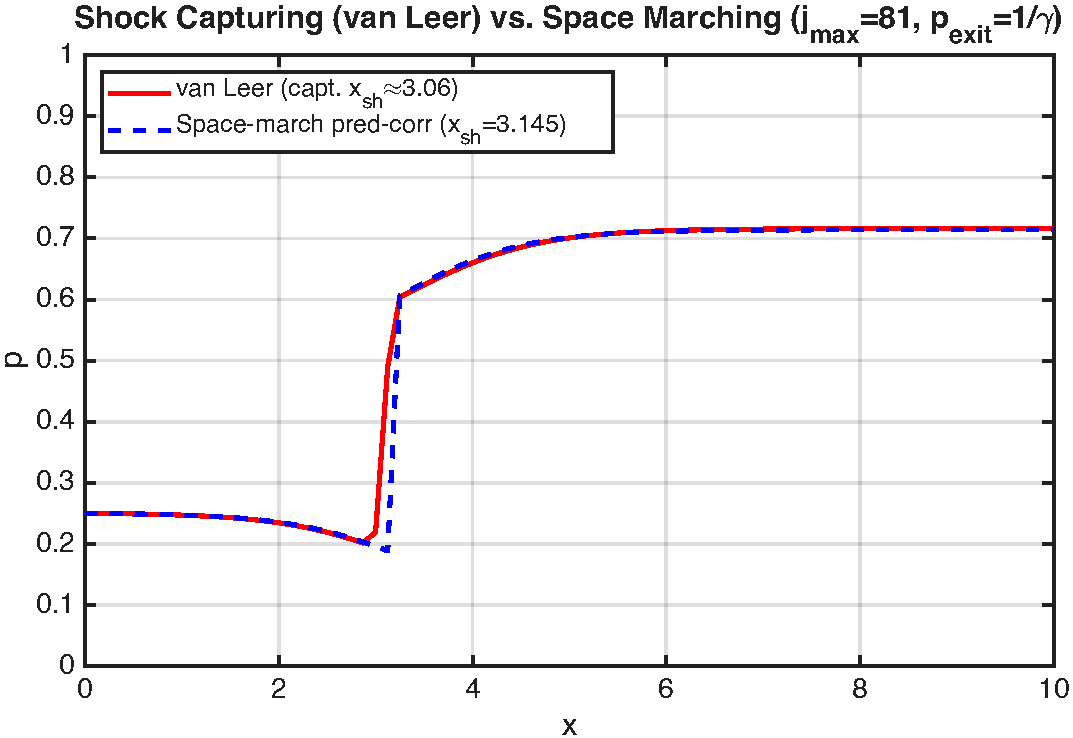
\includegraphics[width=0.65\linewidth]{../outputs/figures/fig06_shockcap_vs_spacemarch_jmax81.pdf}
    \caption{Steady shock-capturing solution (van Leer flux-vector splitting) compared with predictor--corrector space marching, \(j_\text{max} = 81\). The shock-capturing solution smears the discontinuity over two to three cells.}
    \label{fig:results/shockcap/steady-jmax81}
\end{figure}

\begin{figure}[H]
    \centering
    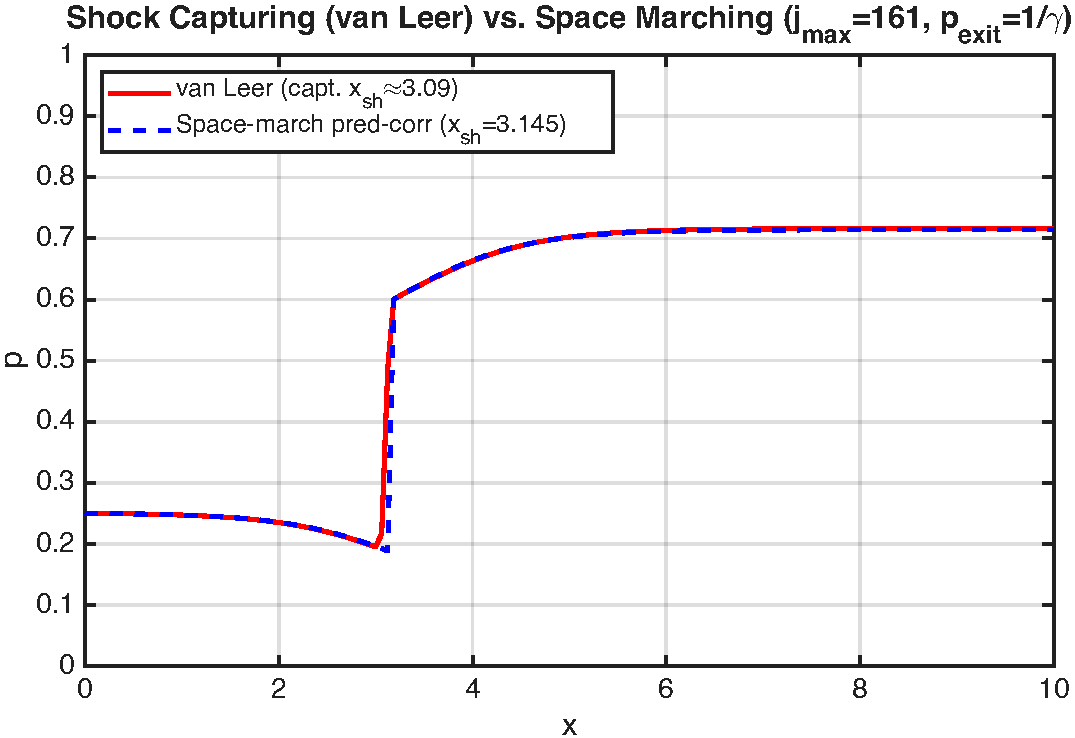
\includegraphics[width=0.65\linewidth]{../outputs/figures/fig07_shockcap_vs_spacemarch_jmax161.pdf}
    \caption{Steady shock-capturing solution (van Leer flux-vector splitting) compared with predictor--corrector space marching, \(j_\text{max} = 161\). The smearing of the captured shock is reduced relative to \cref{fig:results/shockcap/steady-jmax81}.}
    \label{fig:results/shockcap/steady-jmax161}
\end{figure}

\subsubsection{Unsteady Flow} \label{sec:results/shock-capturing/unsteady-flow}

All unsteady cases were initialized with \(x_\text{sh} = 3.125\), a converged steady ramp-up of \(6000\) iterations, and six forced periods of sinusoidal exit-pressure perturbation; sixteen pressure and Mach-number snapshots were saved during the final period to construct the envelopes shown below. The probe location for the time histories is fixed at \(x = x_\text{sh} + 0.05 L = 3.625\), placing it just downstream of the steady-state shock so that any motion of the shock past the probe produces a large pressure swing.

\paragraph{Moderate forcing (\(\Delta p_\text{var} = 0.10\), \(T = 1\)).}
The pressure envelope (\cref{fig:results/unsteady/env-mod}) shows the shock oscillating between roughly \(x \approx 1.7\) and \(x \approx 3.7\) about the steady reference position. The probe history (\cref{fig:results/unsteady/probe-mod}) is approximately periodic after one or two transients, and it is dominated by very rapid swings between roughly \(0.15\) and \(0.78\) as the shock translates past the probe twice per period. The asymmetric, cusp-like waveform reflects the underlying compressible-flow physics: when the shock passes downstream of the probe the probe sees the cold supersonic stream, and when it passes back upstream the probe sees the warm subsonic post-shock stream.

\begin{figure}[H]
    \centering
    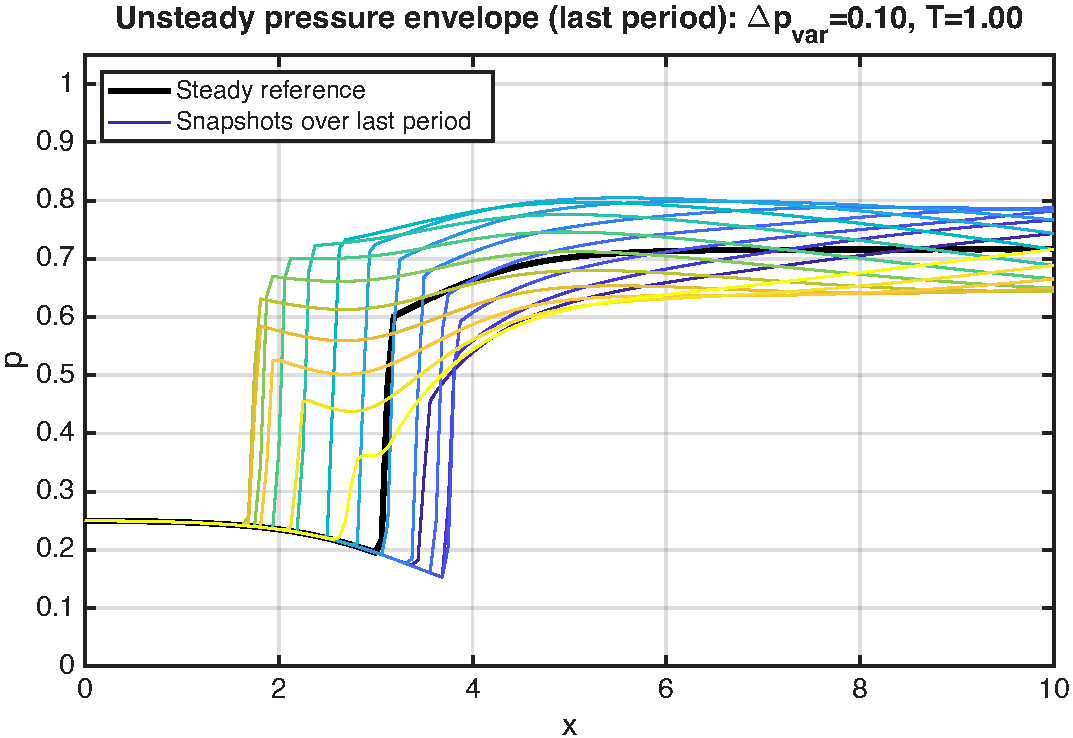
\includegraphics[width=0.65\linewidth]{../outputs/figures/fig08_unsteady_env_mod.pdf}
    \caption{Pressure envelope over the final forced period for the moderate case (\(\Delta p_\text{var} = 0.10\), \(T = 1\), \(j_\text{max} = 161\)).}
    \label{fig:results/unsteady/env-mod}
\end{figure}

\begin{figure}[H]
    \centering
    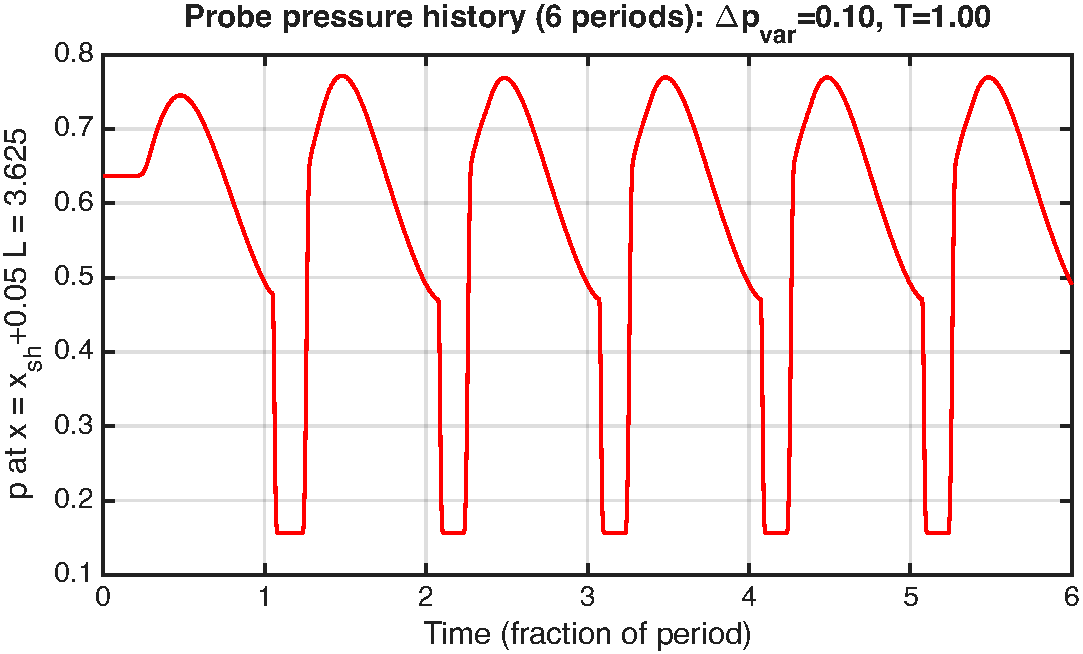
\includegraphics[width=0.65\linewidth]{../outputs/figures/fig09_unsteady_probe_mod.pdf}
    \caption{Pressure history over six periods at the probe \(x = x_\text{sh} + 0.05 L = 3.625\) for the moderate case (\(\Delta p_\text{var} = 0.10\), \(T = 1\)).}
    \label{fig:results/unsteady/probe-mod}
\end{figure}

\paragraph{Long period (\(\Delta p_\text{var} = 0.10\), \(T = 2\)).}
Doubling the forcing period gives the upstream-propagating acoustic disturbance more time to traverse the duct, so the shock has time to follow the boundary condition more closely and excursions are larger. The envelope (\cref{fig:results/unsteady/env-long}) extends from \(x \approx 1.5\) to \(x \approx 4.0\), and the probe history (\cref{fig:results/unsteady/probe-long}) shows a cleaner, more nearly quasi-static waveform than the moderate case. This is essentially the quasi-steady limit: the shock position is nearly in instantaneous equilibrium with the imposed back pressure.

\begin{figure}[H]
    \centering
    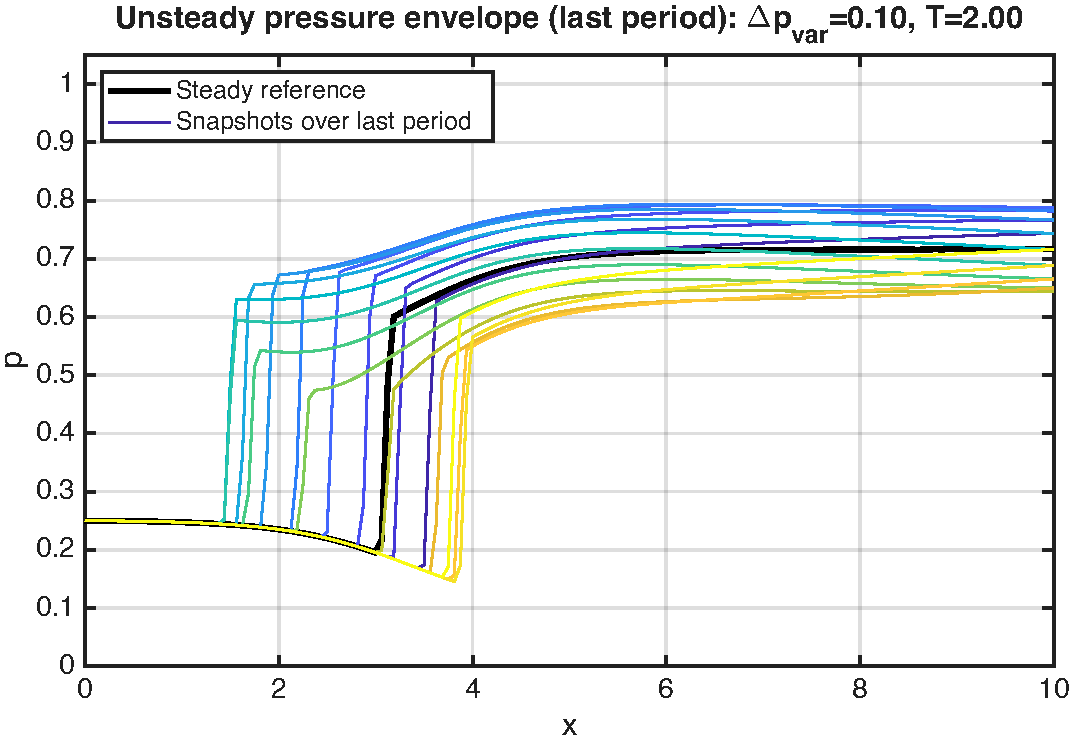
\includegraphics[width=0.65\linewidth]{../outputs/figures/fig10_unsteady_env_long.pdf}
    \caption{Pressure envelope for the long-period case (\(\Delta p_\text{var} = 0.10\), \(T = 2\)).}
    \label{fig:results/unsteady/env-long}
\end{figure}

\begin{figure}[H]
    \centering
    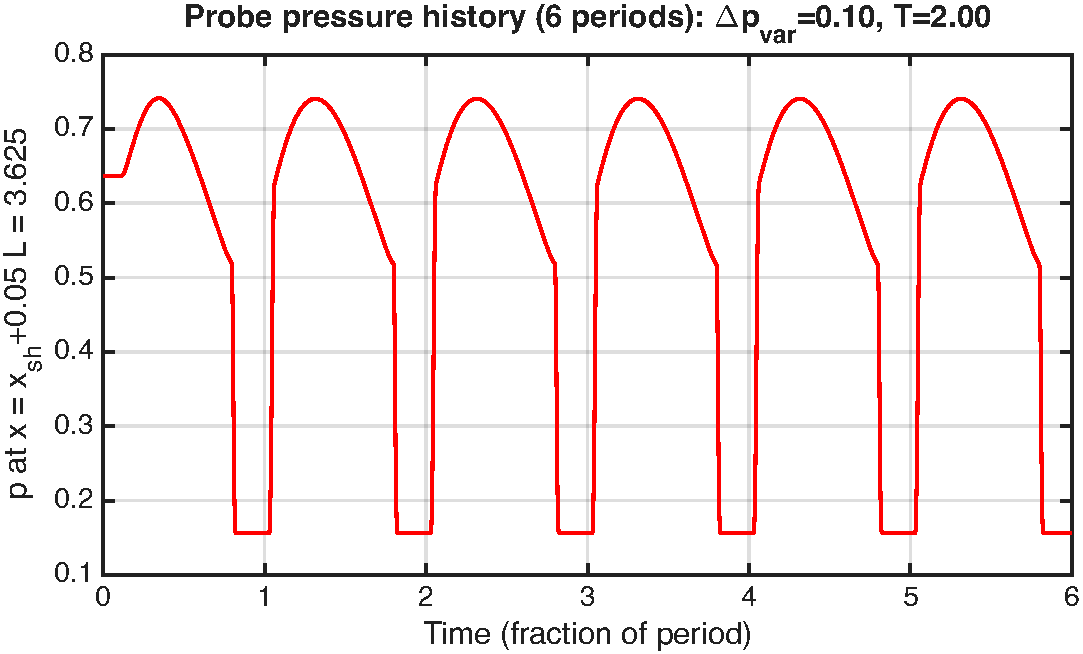
\includegraphics[width=0.65\linewidth]{../outputs/figures/fig11_unsteady_probe_long.pdf}
    \caption{Probe pressure history for the long-period case (\(\Delta p_\text{var} = 0.10\), \(T = 2\)).}
    \label{fig:results/unsteady/probe-long}
\end{figure}

\paragraph{Short period (\(\Delta p_\text{var} = 0.10\), \(T = 1/2\)).}
Halving the period gives the disturbance less time to reach the shock, so the shock motion is reduced relative to the moderate case. The envelope (\cref{fig:results/unsteady/env-short}) is narrower (the shock excursion is roughly \(2.5 \lesssim x \lesssim 3.5\)), and the probe history (\cref{fig:results/unsteady/probe-short}) shows lower amplitude than the moderate case at the same forcing amplitude. Physically, the shock's inertia (its mass-loading by the surrounding flow) acts as a low-pass filter on the imposed boundary condition.

\begin{figure}[H]
    \centering
    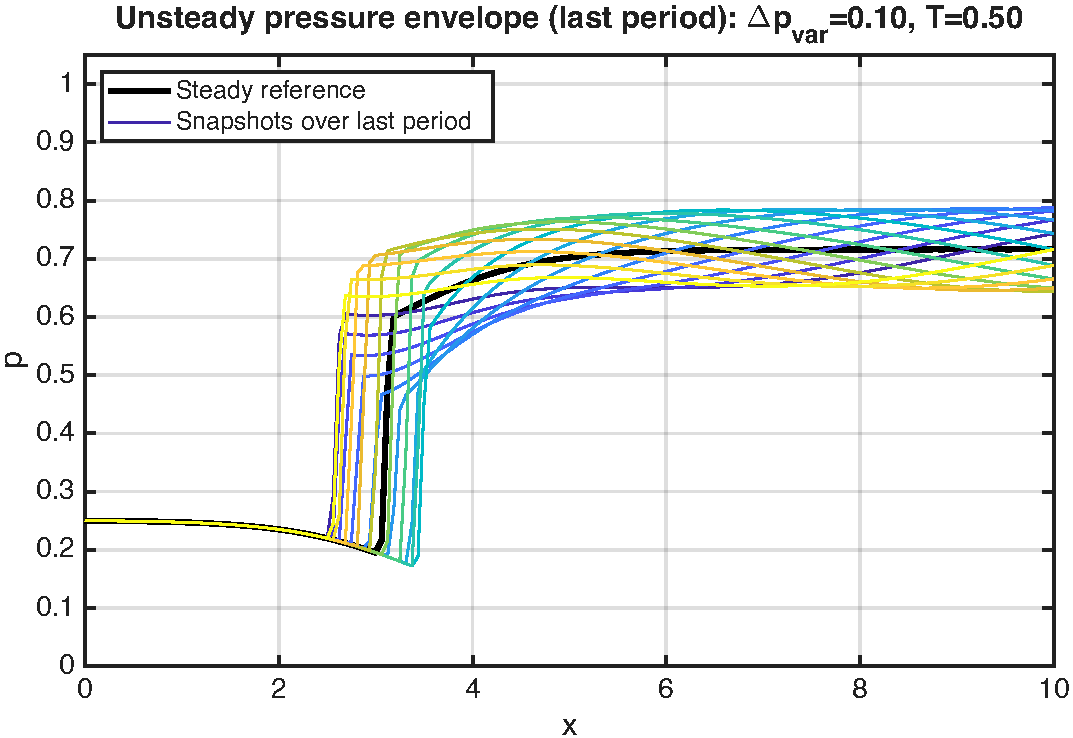
\includegraphics[width=0.65\linewidth]{../outputs/figures/fig12_unsteady_env_short.pdf}
    \caption{Pressure envelope for the short-period case (\(\Delta p_\text{var} = 0.10\), \(T = 1/2\)).}
    \label{fig:results/unsteady/env-short}
\end{figure}

\begin{figure}[H]
    \centering
    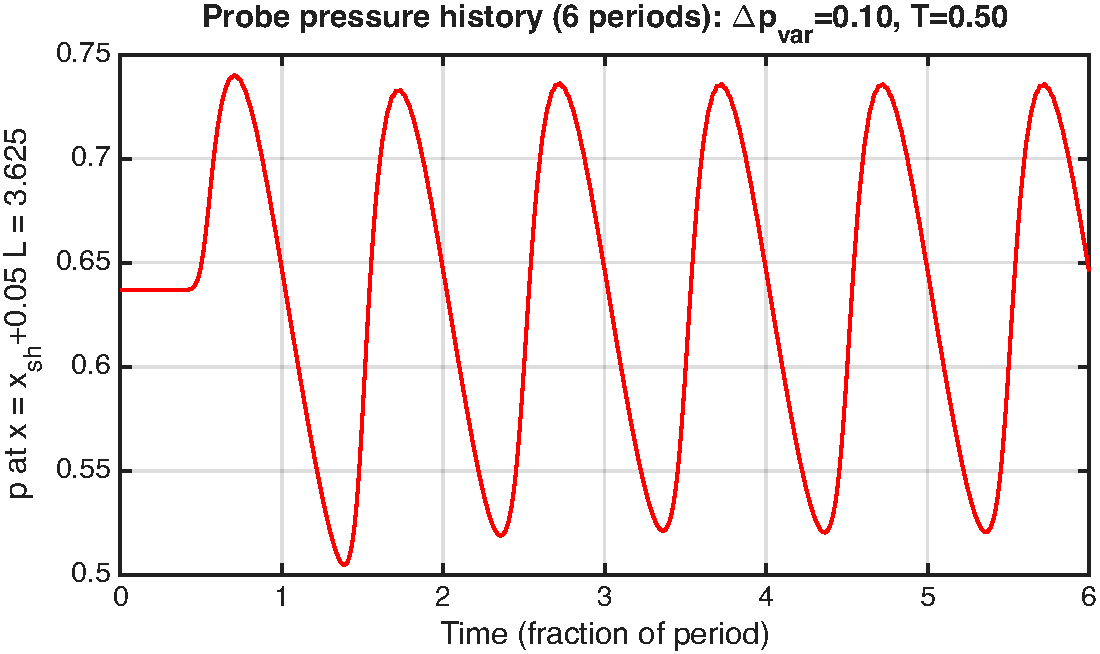
\includegraphics[width=0.65\linewidth]{../outputs/figures/fig13_unsteady_probe_short.pdf}
    \caption{Probe pressure history for the short-period case (\(\Delta p_\text{var} = 0.10\), \(T = 1/2\)).}
    \label{fig:results/unsteady/probe-short}
\end{figure}

\paragraph{Small amplitude (\(\Delta p_\text{var} = 0.02\), \(T = 1\)).}
At one-fifth of the moderate forcing amplitude the response is nearly linear: the envelope (\cref{fig:results/unsteady/env-small}) is tightly clustered around the steady reference, and the probe history (\cref{fig:results/unsteady/probe-small}) is small in amplitude and approximately sinusoidal in shape, rather than exhibiting the cusp-like waveform of the moderate case. The shock excursion is on the order of one to two grid cells. This is the regime in which a perturbation analysis of the steady solution would be expected to be quantitatively accurate.

\begin{figure}[H]
    \centering
    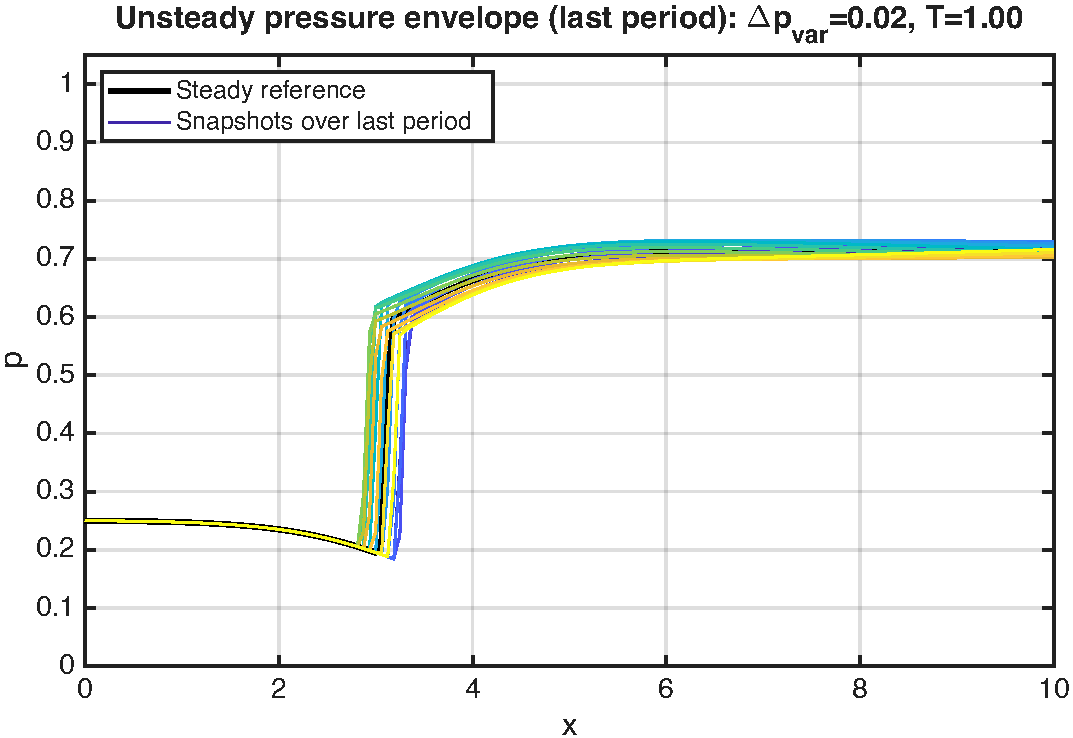
\includegraphics[width=0.65\linewidth]{../outputs/figures/fig14_unsteady_env_small.pdf}
    \caption{Pressure envelope for the small-amplitude case (\(\Delta p_\text{var} = 0.02\), \(T = 1\)).}
    \label{fig:results/unsteady/env-small}
\end{figure}

\begin{figure}[H]
    \centering
    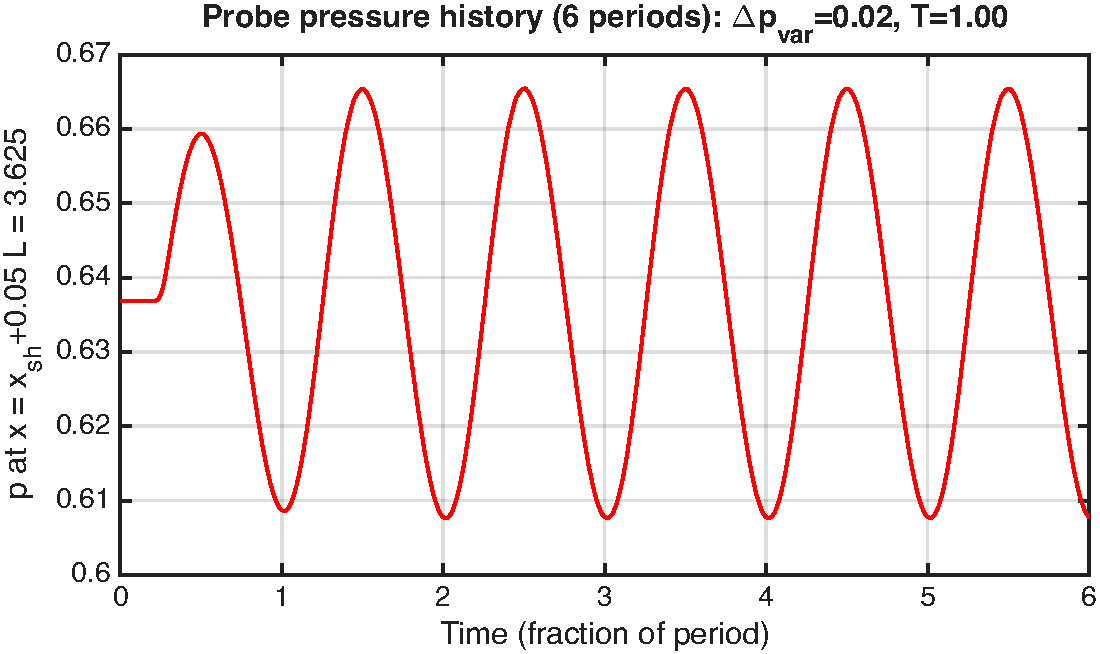
\includegraphics[width=0.65\linewidth]{../outputs/figures/fig15_unsteady_probe_small.pdf}
    \caption{Probe pressure history for the small-amplitude case (\(\Delta p_\text{var} = 0.02\), \(T = 1\)).}
    \label{fig:results/unsteady/probe-small}
\end{figure}

\paragraph{Large amplitude (\(\Delta p_\text{var} = 0.20\), \(T = 1\)).}
Doubling the moderate forcing amplitude pushes the response decisively into the nonlinear regime. The envelope (\cref{fig:results/unsteady/env-large}) shows the shock sweeping over essentially the entire downstream half of the duct, from very near the inlet through approximately \(x \approx 4\); on the upstream excursion the shock reaches close enough to the entrance that the entire supersonic region is briefly compressed against the inlet boundary, and on the downstream excursion the post-shock pressure plateau extends well past \(x = 5\). The probe history (\cref{fig:results/unsteady/probe-large}) shows correspondingly large excursions. In a real device this regime would be associated with violent unsteady loading, possible inlet unstart, and significant total-pressure loss.

\begin{figure}[H]
    \centering
    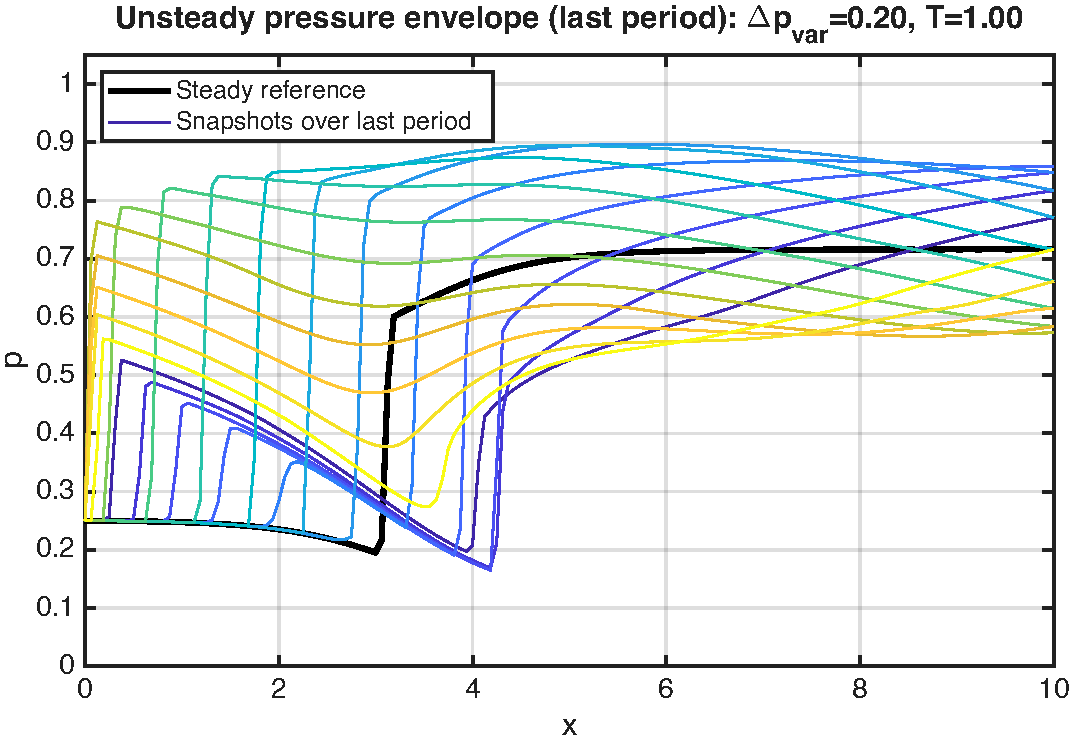
\includegraphics[width=0.65\linewidth]{../outputs/figures/fig16_unsteady_env_large.pdf}
    \caption{Pressure envelope for the large-amplitude case (\(\Delta p_\text{var} = 0.20\), \(T = 1\)). The shock has been driven into a strongly nonlinear regime.}
    \label{fig:results/unsteady/env-large}
\end{figure}

\begin{figure}[H]
    \centering
    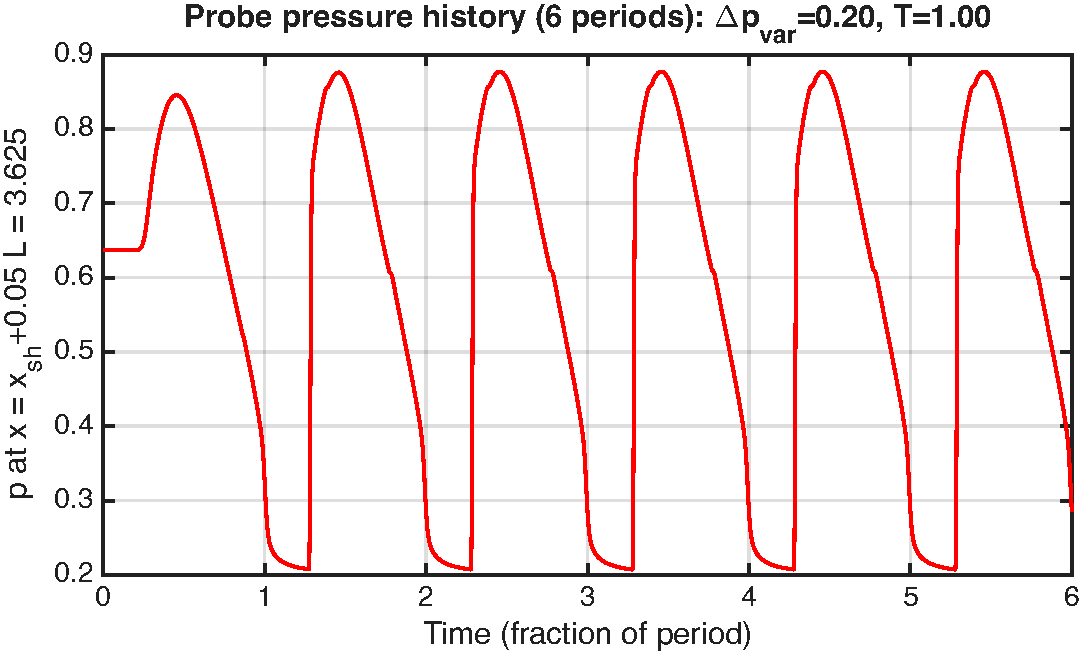
\includegraphics[width=0.65\linewidth]{../outputs/figures/fig17_unsteady_probe_large.pdf}
    \caption{Probe pressure history for the large-amplitude case (\(\Delta p_\text{var} = 0.20\), \(T = 1\)).}
    \label{fig:results/unsteady/probe-large}
\end{figure}

\paragraph{Mach number envelope (moderate case).}
\Cref{fig:results/unsteady/mach-env-mod} plots the Mach-number envelope corresponding to the moderate-case pressure envelope of \cref{fig:results/unsteady/env-mod}. In addition to confirming the shock excursion range visible in the pressure envelope, it shows two pieces of information that the pressure envelope obscures. First, the pre-shock Mach number itself is modulated by the unsteady boundary condition: when the shock is pushed downstream the upstream supersonic expansion proceeds further before the shock and \(M_{1}\) increases (peak \(M_1 \gtrsim 1.8\)), whereas when the shock is pushed upstream \(M_{1}\) is reduced (\(M_1 \approx 1.5\)). Second, the post-shock subsonic Mach distribution shows a wider spread than its pressure counterpart, reflecting the fact that small changes in subsonic pressure correspond to relatively large changes in Mach number through the isentropic-divergence relations. The Mach envelope is therefore a more sensitive diagnostic of the flow's response than the pressure envelope alone.

\begin{figure}[H]
    \centering
    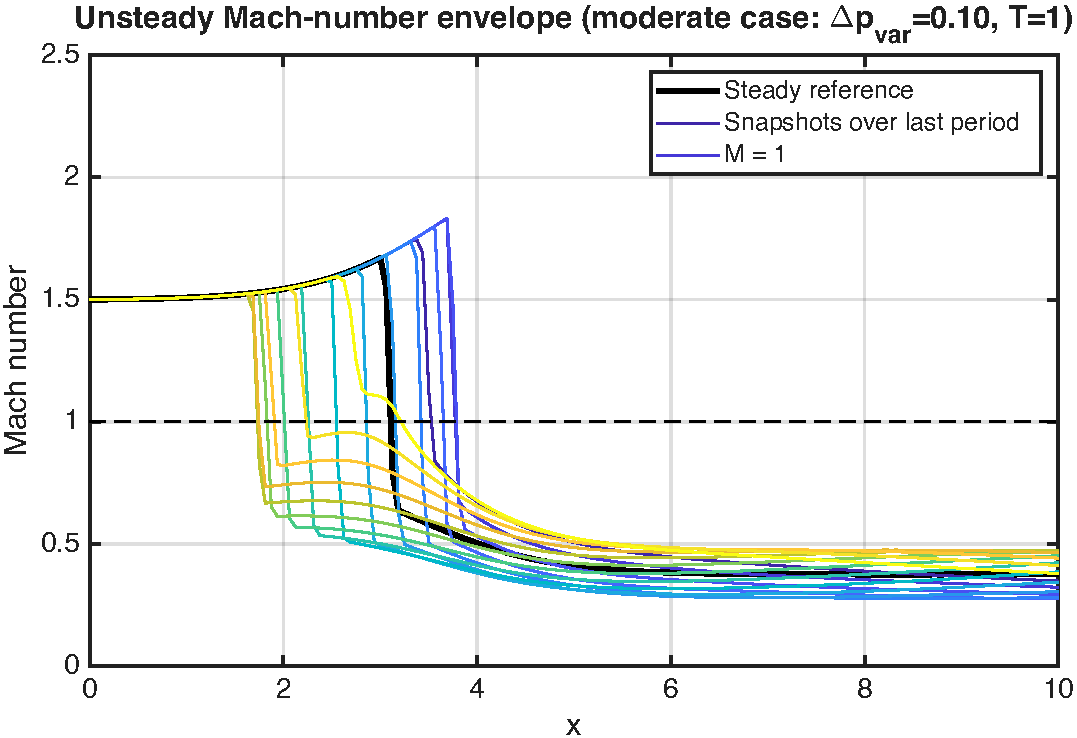
\includegraphics[width=0.65\linewidth]{../outputs/figures/fig18_unsteady_mach_env_mod.pdf}
    \caption{Mach-number envelope for the moderate-case (\(\Delta p_\text{var} = 0.10\), \(T = 1\)). The pre-shock Mach number is modulated between roughly \(M_{1} \approx 1.5\) and \(M_{1} \gtrsim 1.8\) over the period.}
    \label{fig:results/unsteady/mach-env-mod}
\end{figure}

\section{Analysis and Discussion} \label{sec:analysis}

\paragraph{Verification of the space-marching solver.}
The space-marching method has several internal consistency checks available to it. First, mesh refinement: as shown by \cref{fig:results/spacemarch/xsh4-jmax81,fig:results/spacemarch/xsh4-jmax41}, doubling the grid count from 41 to 81 collapses the predictor and predictor--corrector solutions onto each other, indicating that both schemes have converged to within roughly 1\% in the post-shock region by \(j_\text{max} = 81\) and that the predictor--corrector is essentially mesh-converged at \(j_\text{max} = 41\). Beyond mesh refinement, two analytical checks are available: (i)~the upstream supersonic flow obeys the area--Mach relation, so a numerical estimate of \(M(x)\) on the supersonic branch can be compared directly against the closed-form isentropic-flow result; and (ii)~the pressure jump at \(x_\text{sh}\) must satisfy the Rankine--Hugoniot relations to machine precision (this is enforced analytically by \texttt{shock.m}). For external validation, the post-shock pressure recovery in the divergent section can be cross-checked against the isentropic exit-Mach calculation given the post-shock entropy and the fixed exit area ratio.

\paragraph{Verification of the unsteady solver.}
For the unsteady solver, the most informative verification is a steady-state cross-check: setting \(\Delta p_\text{var} = 0\) and converging in time should recover (within mesh resolution) the same shock position and pressure profile as the space-marching solution evaluated at the matching shock location. This was performed for both \(j_\text{max} = 81\) and \(j_\text{max} = 161\) and the agreement was good in both cases (\cref{fig:results/shockcap/steady-jmax81,fig:results/shockcap/steady-jmax161}), with the captured shock position differing from the space-march reference by less than one cell width. Further verification could include a residual-history check (the L\textsubscript{2} norm of \(\Delta \hat Q\) should drop several orders of magnitude during the steady ramp-up before any forcing is applied), a CFL-sensitivity study (halving \(\mathrm{CFL}\) should not change the steady solution but should approximately halve the wall time), and a flux-scheme cross-check (substituting the Steger--Warming or AUSM splitter for van~Leer should yield the same converged solution to within numerical-dissipation differences). For the unsteady cases specifically, the shock-displacement amplitude in the small-perturbation limit (\(\Delta p_\text{var} = 0.02\)) can be compared with a linearized perturbation analysis about the steady-state shock position; the present results suggest a near-linear response in this regime, consistent with such an analysis.

\paragraph{Adequacy of the chosen parameters.}
Of the cases prescribed in the assignment, the moderate-case forcing parameters (\(\Delta p_\text{var} = 0.10\), \(T = 1\)) bracket the most informative regime: the shock excursion is large enough to be physically interesting but not so large that the response is dominated by extreme nonlinearities. The amplitude sweep (small/moderate/large) clearly separates linear, weakly nonlinear, and strongly nonlinear behavior; the period sweep (short/moderate/long) clearly separates the inertia-limited, resonant, and quasi-steady limits. The mesh refinement \(j_\text{max} = 161\) used for the unsteady cases is sufficient to resolve the captured shock to within roughly 0.06 in \(x\), which is small compared to the shock excursion in every case. Six forced periods is enough to wash out the initial transient and produce a periodic envelope. One area that would benefit from additional study is intermediate amplitudes between \(\Delta p_\text{var} = 0.10\) and \(0.20\), since the transition into strongly nonlinear behavior is rather abrupt between those two cases.

\paragraph{What we learned.}
The exercise illustrates that a relatively simple combination of the area--Mach relation, the Rankine--Hugoniot conditions, and the steady-state characteristic boundary conditions captures the entire steady-state phenomenology of transonic flow in a divergent duct, and that adding a flux-vector-split unsteady time-marcher onto exactly the same governing equations yields a tool capable of resolving rich shock-motion physics under unsteady forcing. It also shows the inherent trade-off between shock fitting and shock capturing: shock fitting gives sharper, lower-error solutions for problems with a known shock topology, while shock capturing is geometry-and-topology-agnostic at the cost of cell-scale smearing.

\paragraph{MATLAB versus Python versus C.}
For a problem of this size --- one-dimensional, a few hundred grid points, tens of thousands of time steps --- MATLAB is an excellent choice. Its vectorized arithmetic gives essentially-compiled performance for the inner-loop array updates while keeping the source code very compact (the entire driver and unsteady solver are roughly 250 lines combined). The integrated plotting toolchain produces publication-quality figures with very little ceremony, and the JIT-compiled-on-the-fly model means there is no edit/compile/run cycle to slow down algorithm exploration. Python with NumPy and Matplotlib offers a comparable productivity profile and a much richer general-purpose ecosystem at the cost of slightly higher overhead for very small array operations and a less coherent default plotting story; it would be a strong choice if the same code needed to feed into downstream Python infrastructure (machine-learning models, etc.). C would be by far the fastest at runtime but would multiply the line count and development time several-fold for what is, after all, a teaching exercise; C only really pays for itself when the problem grows to two or three dimensions and the inner loop dominates wall-clock time. For this class, MATLAB is the right choice.

\paragraph{Possible improvements.}
Several extensions to this experiment would strengthen the conclusions. (i)~A higher-order spatial discretization (e.g., MUSCL extrapolation with a slope limiter, or weighted-essentially-non-oscillatory reconstruction) would reduce the smearing of the captured shock. (ii)~A higher-order or implicit time integrator would relax the CFL constraint, which becomes restrictive on fine meshes. (iii)~Using the Roe approximate Riemann solver in place of the flux-vector-split scheme would reduce the numerical dissipation in the post-shock subsonic region, which would in turn allow smaller-amplitude unsteady forcing to be resolved on coarser meshes. (iv)~A formal mesh-refinement study (Richardson extrapolation, observed order of accuracy on a manufactured smooth solution) would put a quantitative number on the discretization error rather than the qualitative comparisons reported here. (v)~Replacing the prescribed sinusoidal exit-pressure forcing with a stochastic or impulse perturbation would expose the natural acoustic modes of the duct and make it possible to identify resonance frequencies. (vi)~Coupling the quasi-1D flow solver to a structural model of the duct walls would allow the simulation of fluid-structure interaction effects, a likely concern for any real propulsion application.

\section{Summary and Conclusions} \label{sec:summary}

A pre-existing MATLAB code base for the analysis of transonic flow in a quasi-1D diverging nozzle was driven through a prescribed matrix of cases and the results were interpreted in light of classical compressible-flow theory. For the steady problem, predictor--corrector space marching was found to be essentially mesh-converged at \(j_\text{max} = 81\), while a predictor-only step shows a measurable error in the post-shock region at \(j_\text{max} = 41\). The exit pressure decreases monotonically with shock position, from \(p_\text{exit} \approx 0.727\) at \(x_\text{sh} = 3.0\) to an asymptote near \(p_\text{exit} \approx 0.480\) as the shock approaches the exit, in agreement with the classical normal-shock-in-divergent-nozzle result. Steady van~Leer shock capturing initialized at \(x_\text{sh} = 3.125\) reproduces the space-marching reference to within one cell width on both the \(j_\text{max} = 81\) and \(j_\text{max} = 161\) grids; the captured shock is smeared over two to three cells, as expected for a flux-vector-split scheme without a high-order reconstruction.

For the unsteady problem, a sinusoidal exit-pressure perturbation drives shock oscillations whose displacement grows with both forcing period and forcing amplitude. The response transitions from a near-linear regime at \(\Delta p_\text{var} = 0.02\) to a strongly nonlinear regime at \(\Delta p_\text{var} = 0.20\), where the shock sweeps over much of the duct length. The Mach-number envelope reveals additional structure not visible in the pressure envelope, in particular the modulation of the pre-shock supersonic Mach number with the imposed back pressure. Across all cases, six forced periods are sufficient to wash out the initial transient and produce a clean periodic envelope.

Looking forward, the main improvements that would tighten these conclusions are higher-order spatial reconstruction and a Roe-type Riemann solver to reduce the numerical dissipation, a formal mesh-refinement study to put quantitative numbers on the discretization error, and an exploration of intermediate forcing amplitudes to characterize the transition into the strongly nonlinear regime more cleanly.

\section{References} \label{sec:references}

\printbibliography[heading=none]

\section{Appendices} \label{sec:appendices}

\subsection{Data} \label{sec:appendices/data}

For the sake of brevity, the raw data will not be displayed in this report. However, in the spirit of completeness, the repository containing the complete data, source code, and notes for this report can be found at \href{https://www.github.com/vaisriv/enae464-lab06}{github:vaisriv/enae464-lab06}.

\subsection{Code} \label{sec:appendices/code}

Similarly, only the code files that are key to the analysis are included below, and can be accessed in full in the aforementioned \href{https://www.github.com/vaisriv/enae464-lab05}{GitHub repository}.

\begin{codeblock}
    \centering
    \caption{Computational Analysis Script.}
    \mintinline{bash}{./src/index.m}
    \inputminted{matlab}{../src/index.m}
    \label{lst:appendices/code/index}
\end{codeblock}

\begin{codeblock}
    \centering
    \caption{Parameterized unsteady-flow solver.}
    \mintinline{bash}{./src/unsteady_run.m}
    \inputminted{matlab}{../src/unsteady_run.m}
    \label{lst:appendices/code/unsteady-run}
\end{codeblock}

% render all references
\nocite{*}

\end{document}
